\section{Sección Uno}
\subsection{Apartado Uno}
\begin{large}
Texto del apartado uno

\begin{itemize}
   \item Item 1
   \item Item 2
   \item Item 3
   \item Item 4
\end{itemize}
\end{large}

\section{Sección Dos}

\begin{large}
\begin{itemize}
   \item Item 1
   \item Item 2
   \item Item 3
\end{itemize}
\end{large}

\section{Sección Tres}

\begin{large}
Bla, bla, bla.
\end{large}

\section{Sección Cuatro}

\begin{large}
Bla, bla, bla.
\end{large}

\newpage

\begin{figure}[htb]
   \centering
   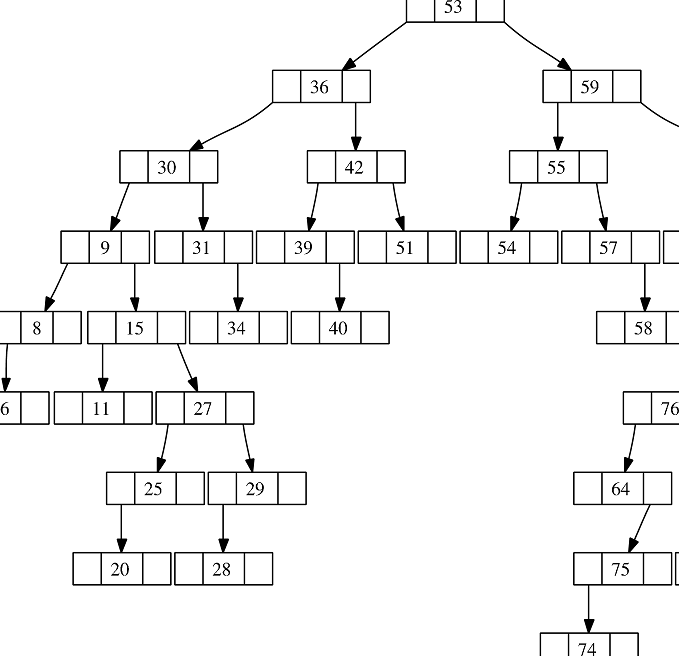
\includegraphics[width=0.8\linewidth]{images/figura_1}
   \caption{Ejemplo de figura}
   \label{chapter:introduction}
\end{figure}